\documentclass{article}
\usepackage[utf8]{inputenc}
\usepackage{amsmath}
\usepackage{amsfonts}
\usepackage{amssymb}
\usepackage{graphicx}
\usepackage{array}
\usepackage{float}
\usepackage{parskip}
\usepackage[table]{xcolor}

\arrayrulecolor[HTML]{b7b7b7}

\title{Modelling Report: Safety Zone around Playground Swings}
\author{Emilia Zabrzanska}
\date{\today}

\begin{document}

\setlength{\parskip}{1em}

\maketitle

\pagebreak

\section*{Specify the Purpose}

This report aims to determine the minimum area required for a safety zone around a playground swing. The goal is to ensure that if a child or an object falls from the swing while it is in motion, the impact and the resulting injuries are minimized.

\section*{Create the Model}

\subsection*{Describe Features Investigated and Outline Mathematics Used}
This model is being used to predict the area required for a safety zone around a set of swings. We will be using a two step approach to determine the length of  the zone, width will not be investigated. Firstly, we model the swing as a pendulum using simple harmonic motion, and find its velocity through conservation of energy. Secondly, we will apply projectile motion principles to determine the distance a child or object travels upon being released from the swing.

\subsection*{State Assumptions}
The model is based on the following assumptions:
\begin{enumerate}
    \item The child or object is modeled as a particle
    \item Motion occurs in two dimensions
    \item The swing is modeled as a rod length \textit{l} 
    \item The swing sits at height \textit{h} above the ground when at rest, such that the distance between the ground and the swing pivot is (\textit{l+h})
    \item The width of the safety zone will the same as the width of the swing supports
    \item The ground is level and perpendicular to the plane of travel
    \item Air resistance and friction are neglected
    \item There are no external forces acting on the swing 
    \item The initial position of the swing will be at  $90^\circ$ to the vertical, with the initial velocity  $v_0 = 0$ $ms^{-1}$  
\end{enumerate}

\subsection*{Variables and Parameters}
Below is a list of all the variables and parameters used in the report, with further clarifications in Fig. 1

\begin{table}[H]
\begin{tabular}{|c|>{\raggedright\arraybackslash}p{0.65\linewidth}|c|}
\hline
Symbol    & Physical Quantity                                                                      & Dimensions \\ \hline
$A$       & Starting position of swing                                                             & $(x,y)$    \\ \hline
$B$       & Final position of swing fall point                                                     & $(x,y)$    \\ \hline
$C$       & Landing point of child/object                                                          & $(x,y)$    \\ \hline
\( \theta_0 \) & Initial angle of the swing when at starting point $A$                                  & Degrees    \\ \hline
\( \theta \)   & Angle when swing is in motion (release point)                                          & Degrees    \\ \hline
$w$       & Width of the swing safety landing zone                                                 & $m$        \\ \hline
$H_A$   & Height from the ground to the top of the swing pivot and swing at point $A$&    $m$        \\   \hline
$H_B$   &  Height from the ground to the swing at point $B$     &$m$        \\  \hline
$l$       & Length of the swing rod, from seat to pivot                                            & $m$        \\ \hline
$h$       & Height from ground to swing seat when vertical and at rest                             & $m$        \\ \hline
$D$       & Total distance from swing centre point, $O$, to where the child/object hits the ground & $m$        \\ \hline
$d_s$     & Horizontal distance from swing centre $O$ to release point, $B$                        & $m$        \\ \hline
$d_f$     & Horizontal distance travelled during fall, from release point $B$ to landing point $C$ & $m$        \\ \hline
$s$     & Arbitrary height      &$m$        \\  \hline
$t$       & Time of flight                                                                         & $s$        \\ \hline
$g$       & The magnitude of the acceleration due to gravity                                       & $ms^{-2}$  \\ \hline
$m$       & Mass of the child/object                                                               & $kg$       \\ \hline
$v$       & Magnitude of the velocity of the child/object                                          & $ms^{-1}$  \\ \hline
$v_A$       & Magnitude of the velocity of the child/object at point $A$                                          & $ms^{-1}$  \\ \hline
$v_B$       & Magnitude of the velocity of the child/object at point $B$                                         & $ms^{-1}$  \\ \hline
$E$       & Total mechanical energy of the system                                                  & $J$        \\ \hline
$U$       & Potential energy of the system                                                         & $J$        \\ \hline
$T$       & Kinetic energy of the system                                                           & $J$        \\ \hline
\end{tabular}
\caption{Variable and Parameter list}
\label{tab:my_table}
\end{table}

\begin{figure}[ht]
    \centering
    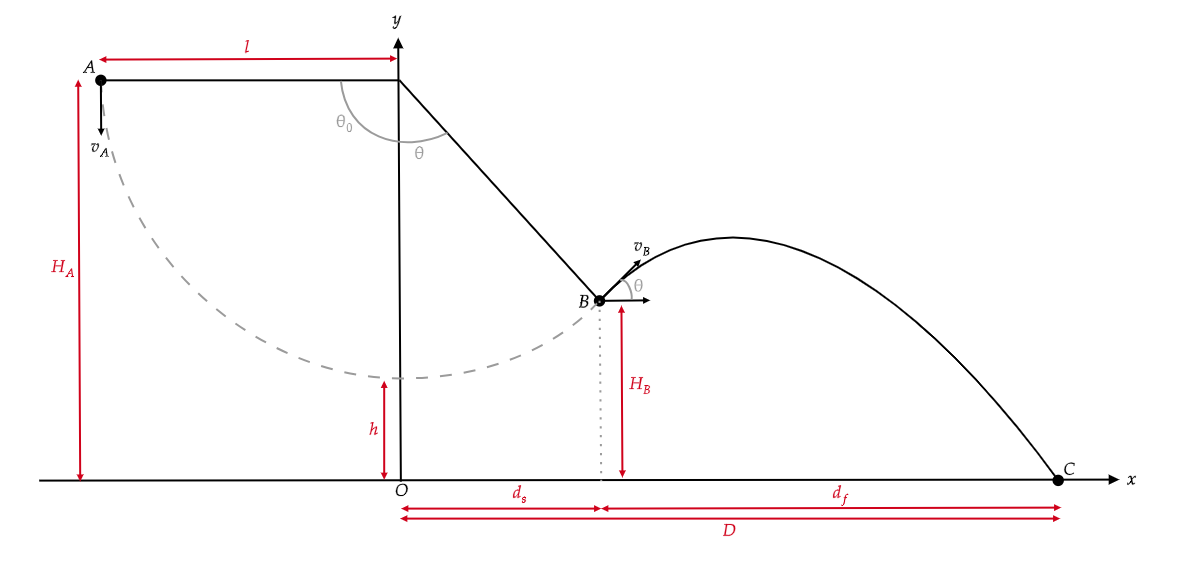
\includegraphics[width=1.00\linewidth]{Fig 1.png}
    \caption{Complete system}
    \label{fig: Swing diagram}
\end{figure}

\subsection*{Formulate Mathematical Relationships}

\subsubsection*{Part 1: Pendulum}

\begin{figure}[H]
    \centering
    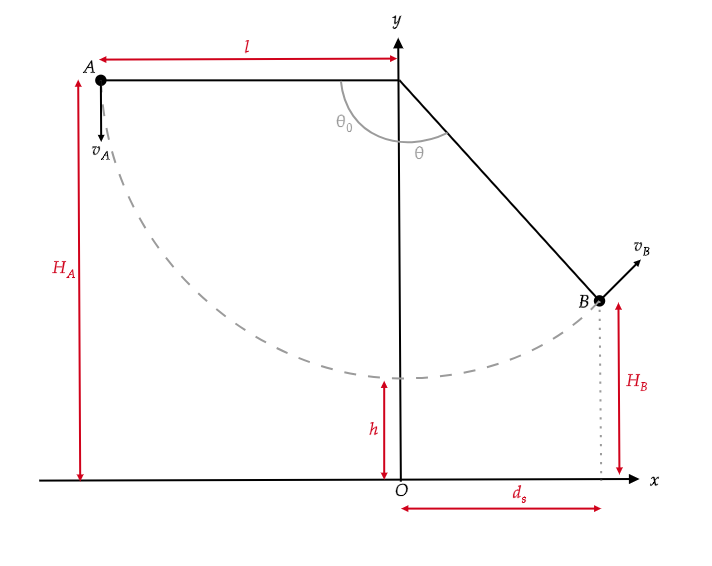
\includegraphics[width=0.70\linewidth]{Fig 2.png}
    \caption{Pendulum}
    \label{fig: Pendulum diagram}
\end{figure}

We first use conservation of energy to compare the Total Mechanical Energy from our start point, $A$, to the point at which the child/object falls from the swing, $B$\footnote{As per points 8, 9 and 11 on Page 67 of the Handbook}. We will use this relationship to find the velocity at the point the child/object leaves the swing.
\par
\noindent By using Assumptions $(1), (2), (3), (4), (6), (7), (8)$ we know that the total mechanical energy, E, is conserved.
\par
\noindent We can therefore use the following: 
\begin{equation}
    E = U + T
\end{equation}

where the Potential Energy $U$ for some arbitrary height $s$ can be expressed as

\[ U = mgs \]

and Kinetic energy can be found using

\[ T = \frac{1}{2} mv^2 \]

\par
\noindent Using conservation of energy allows us to formulate the following expression:

\[ E_A = E_B \]
\begin{equation}
    \Rightarrow mgH_A + \frac{mv_A^2}{2} = mgH_B + \frac{mv_B^2}{2}
\end{equation}

simplifying further by dividing through by $m$ gives us 

\[ gH_A + \frac{v_A^2}{2} = gH_B + \frac{v_B^2}{2}\]

As per assumptions $(7), (8)$ and $(9)$, we take $v_A = 0$, therefore giving us

\[ gH_A = gH_B + \frac{v_B^2}{2}\]

which can be simplified even further to retrieve an expression for $v_B$

\[ gH_A - gH_B = \frac{v_B^2}{2}\]
\[\Rightarrow 2(gH_A - gH_B) = v_B^2\]
\begin{equation}
    \Rightarrow 2g(H_A - H_B) = v_B^2
\end{equation}

We can now express $H_A$ and $H_B$ in terms of the swing rod length $l$ and the height from the ground to the swing $h$, as per assumptions $(3), (4), (6)$

\[H_A = l + h \]
\[H_B = l + h - lcos(\theta) \]

Therefore, the expression for $H_A - H_B$ becomes

\[H_A - H_B = l + h - (l + h - lcos(\theta) \]
\begin{equation}
    \Rightarrow H_A - H_B = lcos(\theta)
\end{equation}

We can now substitute this into our expression for $v_b^2$:

\[v_B^2 = 2g(H_A - H_B)\]
\[\Rightarrow v_B^2 = 2glcos(\theta)\]

Our final expression for $v_B$ will therefore be 

\begin{equation}
    v_B = \pm \sqrt{2glcos(\theta)}
\end{equation}

where only the positive value will be considered.
\par
\noindent We have now found our value for the magnitude of velocity at the point in the swing where the child/object falls. As per assumption $(8)$ we can state that due to there not being any external forces acting on the swing, the child/object will leave the swing with the same velocity as $v_B$, allowing us to move onto Part 2 of our model. 

\subsubsection*{Part 2: Projectile Motion}

\begin{figure}[H]
    \centering
    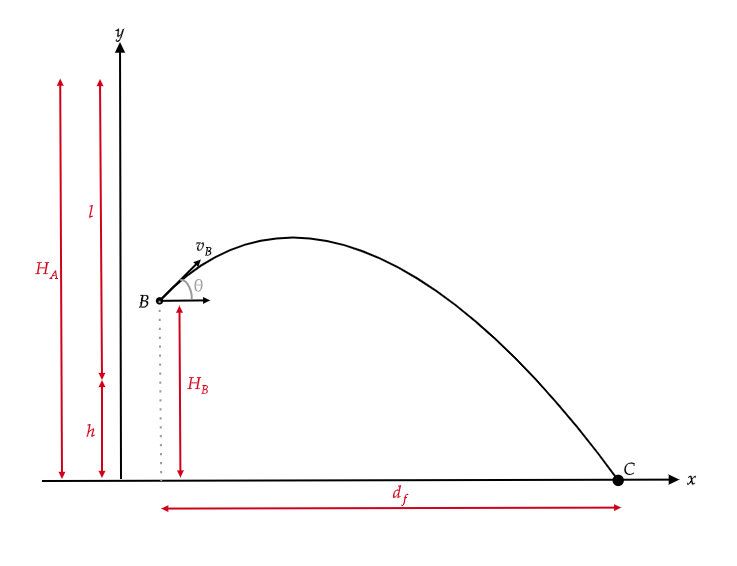
\includegraphics[width=0.70\linewidth]{Fig 3.png}
    \caption{Projectile motion}
    \label{fig: Projectile motion diagram}
\end{figure}

Having concluded the initial speed of our projectile will be will be the same as that of the child/object at point $B$ on the swing, we are now able to find an expression for the total distance travelled, $D$
\par
\noindent As shown in Figure 1, we can express $D$ as:

\begin{equation}
    D = d_s + d_f
\end{equation}

$d_s$ can be found through simple trigonometric calculations based on the length of the swing rod as illustrated in Figure 2

\begin{equation}
    d_s = lsin(\theta)
\end{equation}

we then find $d_f$ through the equations of motion\footnote{As per point 7 on Page 37 of the Handbook}, where $v_{Bx}$ is the horizontal component of the magnitude of velocity at $B$ and $t$ is the time taken for the child/object to hit the ground. It is important to note that our acceleration due to gravity, $g$, is negative here, as we are following the downwards motion of the particle.

\begin{equation}
    d_f = v_{Bx}t
\end{equation}

and $t$ is found using

\begin{equation}
    y = H_B + v_{By}t - \frac{gt^2}{2}
\end{equation}

Once an expression for $t$ is obtained, we will substitute back to fine $D$

\[D = lsin(\theta) + v_{Bx}t\]

It is important to note that this is only the length travelled from the centre of the swing, $O$, to the point at which the child/object hits the ground, $C$. As the child or object can fall off the swing in either direction, the safety zone must have a length of $2D$, a distance of $D$ either side of the swing.
\par
\noindent Having found this length, we are able to propose an area for our safety zone. By assumption $(5)$, the width of our safety zone is $w$, so our total area will be

\begin{equation}
    Area = 2Dw
\end{equation}

\section*{Do the Mathematics}

\subsection*{Derive a first model}

To accurately provide an expression for the area of our swing safety zone, we must find an expression for the distance travelled from the midpoint of the swing, $O$, to the point at which the child or object makes contact with the ground at $C$. We will then duplicate this to find the total length $2D$.

As per equations $(6), (7)$, and $(8)$, this distance can be found by 

\[D = d_s + d_f\]
where 
\[d_s = lsin(\theta)\]
\[d_f = v_{Bx}t\]

We first need to find the time taken for the child/object to fall to the ground (Point $C$), so using equation $(9)$ and taking $y = 0$ will give us 

\[0 = H_B + v_{By}t - \frac{gt^2}{2}\]
\[\Rightarrow \frac{gt^2}{2} - v_{By}t - H_B = 0\]

this expression can now be solved for $t$ using the quadratic formula

\[ t = \frac{v_{By} \pm \sqrt{v_{By}^2 + 2gH_B}}{g}\]

where we will take the positive value as $t>0$.
\par
\noindent This gives us a final value for $t$ 

\begin{equation}
    t = \frac{1}{g}(v_{By} + \sqrt{v_{By}^2 + 2gH_B})
\end{equation}

\par
\noindent Our next step will be to find a final expression for $d_f$ from which we can then derive our total distance.

\[d_f = v_{Bx}t\]
\[ \Rightarrow d_f = \frac{1}{g}v_{Bx}(v_{By} + \sqrt{v_{By}^2 + 2gH_B})\]

To simplify this expression we evaluate $v_B$ into its components using trigonometry, as shown in Figure 3.

\[v_{Bx} = \sqrt{2glcos(\theta)}cos(\theta)\]
\[v_{By} = \sqrt{2glcos(\theta)}sin(\theta)\]

Using these expressions, alongside the value previously found for $H_B$, we can now substitute everything into equation $(8)$

\[d_f = \frac{1}{g} \sqrt{2glcos(\theta)}cos(\theta) ( \sqrt{2glcos(\theta)}sin(\theta) + \sqrt{(\sqrt{2glcos(\theta)}sin(\theta))^2 + 2g(l + h - lcos(\theta))}) \]

\pagebreak

This can then be expanded and simplified as follows

\begin{flalign*}
d_f & = \frac{1}{g} \sqrt{2glcos(\theta)}cos(\theta) ( \sqrt{2glcos(\theta)}sin(\theta) + \sqrt{2glcos(\theta)sin^2(\theta) + 2g(l + h - lcos(\theta))}) &\\
   & =  \frac{1}{g} \sqrt{2glcos(\theta)}cos(\theta) ( \sqrt{2glcos(\theta)}sin(\theta) + \sqrt{2glcos(\theta)(sin^2(\theta) - 1) + 2gl +2gh}) &\\
   & = \frac{1}{g} \sqrt{2glcos(\theta)}cos(\theta) ( \sqrt{2glcos(\theta)}sin(\theta) + \sqrt{-2glcos^3(\theta) + 2gl +2gh}) &\\
   & = \frac{1}{g}cos(\theta) (2glcos(\theta)sin(\theta) + \sqrt{-4g^2l^2cos^4(\theta) + 4g^2l^2cos(\theta) +4g^2hlcos(\theta)}) &\\
   & = \frac{1}{g}cos(\theta) (2glcos(\theta)sin(\theta) + 2g\sqrt{-l^2cos^4(\theta) + l^2cos(\theta) +hlcos(\theta)}) &\\
   & = 2lcos^2(\theta)sin(\theta) + 2cos(\theta)\sqrt{hlcos(\theta) + l^2cos(\theta) - l^2cos^4(\theta)} &\\
\end{flalign*}

\noindent Having now found an expression for both $d_s$ and $d_f$, our total distance from the mid point of the swing can now be found, from equation $(6)$

\begin{equation}
    D = lsin(\theta) + 2lcos^2(\theta)sin(\theta) + 2cos(\theta)\sqrt{hlcos(\theta) + l^2cos(\theta) - l^2cos^4(\theta)}
\end{equation}

\subsection*{Draw graphs showing typical relationships}
Taking $l$ and $h$ as constants, we can plot a graph of $D$ against $\theta$ to evaluate the relationship between them. As shown in Figure 4, the function has a single maximum, illustrated by the red line to be in the range of $30^\circ < \theta < 40^\circ$.

\begin{figure}[H]
    \centering
    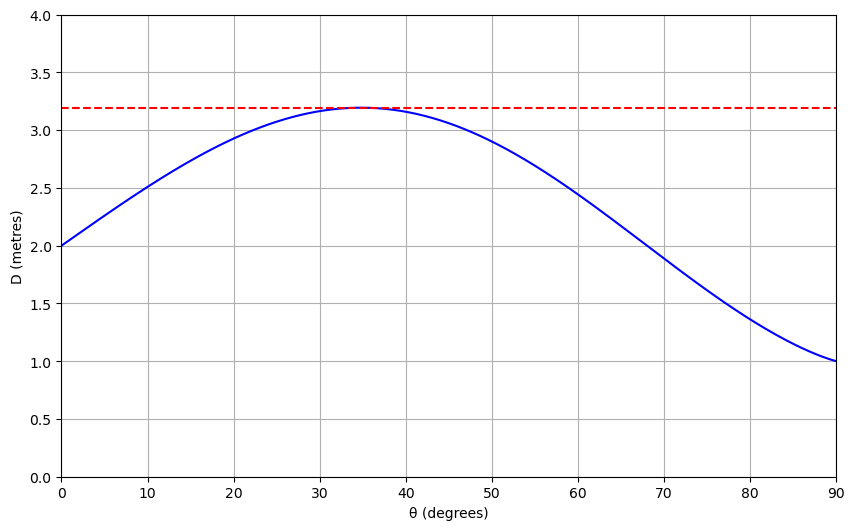
\includegraphics[width=0.70\linewidth]{Fig 4.png}
    \caption{Graph of $D$ against $\theta$ }
    \label{fig: Graph}
\end{figure}

We can therefore imply the value for $D$ will be at its maximum when the child or object leaves the swing when the angle is within this range.

\subsection*{Check your model using dimensional analysis}

We must now check the dimensions of our final formula for the length of the safety zone, equation $(12)$, which is as follows:

\[D = lsin(\theta) + 2lcos^2(\theta)sin(\theta) + 2cos(\theta)\sqrt{hlcos(\theta) + l^2cos(\theta) - l^2cos^4(\theta)}\]

From Table 1, we take the units of $l$ and $h$ to both be metres/$m$, whereas $\theta$ is dimensionless. This allows us to find the dimensions of $D$ to be

\begin{flalign*}
    D & = [m] + [m] + \sqrt{ [m][m] + [m]^2 + [m]^2 } &\\
    & = [m] + [m] + \sqrt{ [m]^2 } &\\
    & = [m] + [m] + [m] &\\
    & = [m] &\\
\end{flalign*}

The dimensions of $D$ correctly simplify to be metres, as required.

\section*{Interpret the Results}

\subsection*{Collect relevant data for parameter values}
From equation $(12)$, our equation for $D$, our parameters are $l$, $h$ and $\theta$

The British and European Standard for playground equipment and surfacing is BS EN 1176.

From this, we will assume that $h = 0.35$\footnote{As stated in EN 1176, the minimum seat ground clearance in the rest position must be $0.35m$}, which will change equation $(12)$ to

\small
\begin{equation}
    D = lsin(\theta) + 2lcos^2(\theta)sin(\theta) + 2cos(\theta)\sqrt{0.35lcos(\theta) + l^2cos(\theta) - l^2cos^4(\theta)}
\end{equation}
\normalsize

We can now calculate our maximum vales for $D$ and $\theta$ by substituting different $l$ values into our equation.

\subsection*{Describe the mathematical solution }
In this model, I will consider values of $l$ ranging from $2.0 - 4.0m$, all expressed in Table 2.

To calculate these, I went through the following steps:

Take $l = 2.0m$, equation $(13)$ will now become 

\begin{flalign*}
    D & = 2sin(\theta) + 4cos^2(\theta)sin(\theta) + 2cos(\theta)\sqrt{0.70cos(\theta) + 4cos(\theta) - 4cos^4(\theta)} &\\
    & = 2sin(\theta) + 4cos^2(\theta)sin(\theta) + 2cos(\theta)\sqrt{4.70cos(\theta) - 4cos^4(\theta)}
\end{flalign*}

To find $D_{max}$, we must find the critical points of the function and classify them. To do this, we evaluate where $D_{max}'(\theta) = 0$. For $l = 2.0m$, this gives us a value of $\theta_{max} = 39.1^\circ$

We can now substitute our $\theta_{max}$ value back into our expression for $D$ to give us our value for $D_{max}$, which is $5.08m$ for $l = 2.0m$.

Following a similar method, we can find $D_{max}$ and $\theta_{max}$ for other values of $l$. I have included a value for $2D_{max}$, which gives us our value for the total length of our Safety Zone, accounting for a fall from either end of the swing.


\begin{table}[H]
    \centering
    \begin{tabular}{|c|c|c|c|} \hline 
         $l/m$&  $\theta_{max}/degrees$&  $D_{max}/m$& $2D_{max}$\\ \hline
         $2.0$&  $39.1^\circ$&  $5.08$& $10.2$\\ \hline
         $2.5$&  $39.5^\circ$&  $6.28$& $12.6$\\ \hline
         $3.0$&  $39.7^\circ$&  $7.48$& $15.0$\\ \hline
         $3.5$&  $39.9^\circ$&  $8.68$& $17.4$\\ \hline
         $4.0$&  $40.0^\circ$&  $9.87$& $19.8$\\ \hline
    \end{tabular}
    \caption{Maximum Values}
    \label{tab:Max values}
\end{table}

\subsection*{Find predictions to compare with reality}
According to the guidance mentioned previously, EN 1176, the minimum safety zone length for a set of swings should be as stated 

\textit{\noindent Surfacing requirements: Free Fall height is calculated from the centre of the stationary seat surface at $60^\circ$ forward and back, where there are different areas for synthetic and loose-fill surfaces in a box or pit:}
\par
\textit{synthetic: $sin(60^\circ)$ x length of suspension member + 1.75m}
\par
\textit{loose-fill: $sin(60^\circ)$ x length of suspension member + 2.25m}

Taking the worst case scenario, we will compare our data to the equation

\begin{equation}
    sin(60^\circ)h + 2.25
\end{equation}

\section*{Evaluate the Model}

\subsection*{Collect data to compare with the model }

As seen in Figure 5, an EN 1176 compliant swing by The Playground Centre has a total height of $2.20m$ and a safety zone of $7.62m$. 

\begin{figure}[H]
    \centering
    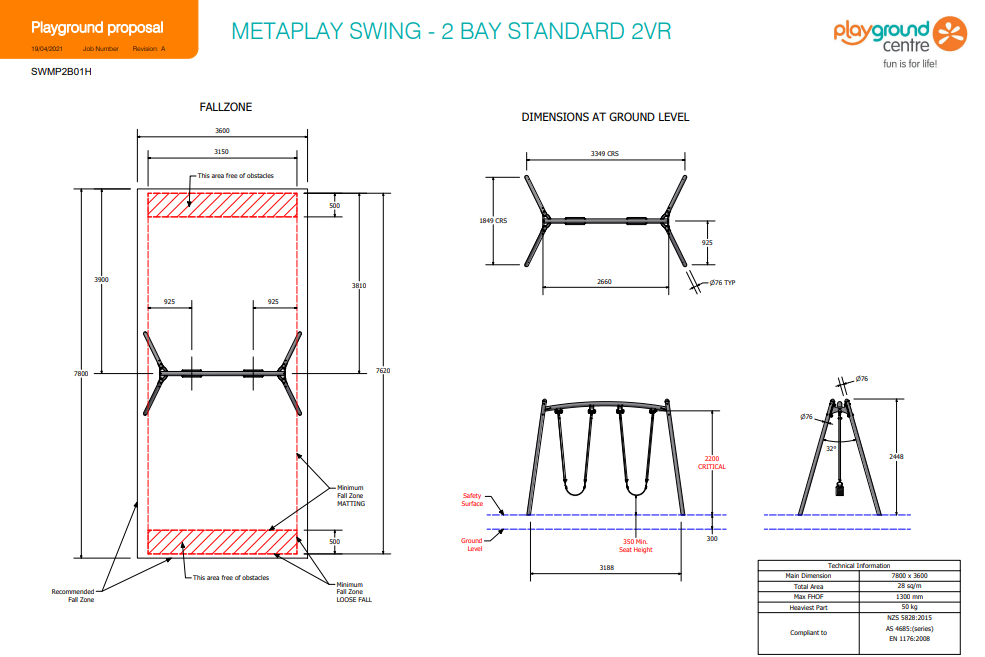
\includegraphics[width=0.70\linewidth]{Fig 5.png}
    \caption{Comparison to real swing }
    \label{fig: Swing}
\end{figure}

\subsection*{Test your first model }
Comparing my model predictions to the data given by the swing manufacturer, the model gives a much longer length than actually required. We have been considering the worst case scenarios for our model, therefore arising greater values than necessary in most cases. 

\subsection*{Criticise your first model }
My model is calculating lengths greater than required, and is very complicated in terms of the formulas and equations used, as in equation $(12)$. I believe the formulas could be simplified to make seamless calculations easier and faster for different heights of the swing, as well as adjusting certain variables to make the predictions more aligned with real values. 

\subsection*{Review your assumptions}
I believe the following assumptions need changing:
\par
\noindent $(1)$ The dimensions of the child need to be taken into consideration.
\par
\noindent $(2)$ Motion will be in more than one direction, due to wind and other influences.
\par
\noindent $(7), (8)$ There will be other forces acting on the swing, which all must be considered.

\section*{Revise the Model}

\subsection*{Decide whether to revise your first model}
I believe a revision to the model is necessary, due to the length predicted being incorrect, and new factors needing to be taken into consideration. As seen in the evaluation, the model does not align with real data. By considering factors that reflect reality such as all external fores and and dimensions of the child or object falling off the swing, the maximum distance travelled will be greatly reduced, as the fall will be slowed down a lot faster.

\subsection*{Describe your intended revision}
Assumptions $(1), (7)$ and $(8)$ will be changed to the following.
\par
Assumption $(1)$ will be : \textit{The length and width of the child or object will be considered}.
\par
Assumption $(7)$ will be : \textit{Air resistance and Friction will be considered}.
\par
Assumption $(8)$ will be : \textit{All external forces acting on the swing will be taken into consideration}.

\section*{Conclusions}

\subsection*{Summarise your modelling}
Overall, the first model was successful in predicting a safe landing zone for the child/object, but due to no external influences acting on the swing, the distance travelled was much greater than required. This is due to there not being any other factors to affect the projectile motion, leading to a maximised value of $D$. By revising our model to consider new factors such as air resistance and friction, the child or object falling will slow down and fall much quicker, helping our data align with that of reality and make the model more successful.

\end{document}
